\documentclass{article}
\newcommand{\singleline}{\hrule height 0.8pt}
\newcommand{\mydate}{Otctober 2, 2025 - \today}
\newcommand{\mytitle}{Quantum Mechanics Technology Processing and Conclusions}
\title{\textbf{\mytitle}}
\author{Jiete XUE}
\date{\mydate}
\usepackage{fancyhdr}
\pagestyle{fancy}
\fancyhf{}
\fancyhead[L]{\leftmark}
\fancyfoot[C]{\thepage}
\usepackage[perpage]{footmisc}
\usepackage{tocloft}
\renewcommand{\cftsecleader}{\cftdotfill{\cftdotsep}}
\usepackage{tcolorbox}
\definecolor{mlv}{RGB}{40, 137, 124}
\usepackage[colorlinks=true, linkcolor=mlv, citecolor=red, urlcolor=cyan, filecolor=mlv]{hyperref}
\usepackage{amsthm}
\usepackage{amsmath}
\usepackage{amssymb}
\usepackage{mathrsfs}
\usepackage{physics}
\usepackage{tikz}
\usepackage{tcolorbox}
\usepackage{graphicx}
\graphicspath{{./}{images/}}
\usepackage{float}

%% 右矢
%\ket{\psi}          % 输出:|ψ⟩
%\ket{\psi(t)}       % 输出:|ψ(t)⟩
%
%% 左矢
%\bra{\phi}          % 输出:⟨φ|
%
%% 期望值
%\expval{\hat{A}}    % 输出:⟨Â⟩
%\expval{\hat{A}}{\psi}  % 输出:⟨ψ|Â|ψ⟩
%
%% 对易子
%\comm{\hat{A}}{\hat{B}}  % 输出:[Â, B̂]

\usepackage{pdfpages}

\newtheoremstyle{1}{}{}{}{}{\bfseries}{}{\newline}{}
\newtheoremstyle{2}{}{}{}{}{\bfseries}{.}{\newline}{}
\theoremstyle{1}
\newtheorem{problem}{Problem}[section]
\newtheorem{theorem}[problem]{Theorem}
\usepackage{chngcntr}
\counterwithin{equation}{section}
\counterwithin{figure}{section}
\newcommand{\pa}{\partial}
\newcommand{\ii}{\mathrm{i}}
\newcommand{\ee}{\mathrm{e}}

\begin{document}
\maketitle
\thispagestyle{empty}
\newpage
\pagenumbering{roman}
\setcounter{page}{1}
\tableofcontents
\newpage
\pagenumbering{arabic}
\setcounter{page}{1}





\section{Quantization}
\begin{equation}\label{eq 1.1}
    \oint p\dd{q}=n h +C,\ n=1,2,3,\dots 
\end{equation}
This is not always right, but it's a good approximation. 
\section{Heisenberg's Breakthrough}
Heisenberg use matrices to represent quantum states.\footnote{Here use the similar notation $x(t)$ and $x$, but they represent different things. In some cases, we will ignore $(t)$ but still represent $x(t)$ for convenience.}
\begin{equation}
    x_{n,m}(t)=x_{n,m}\ee^{\ii\omega_{n,m}t}.
\end{equation}
With the \textbf{Ritz combination law}\footnote{You can imagine a electron moving from state $m$ to state $n$ passing state $k$.}
\begin{equation}
    \omega_{n,m}=\omega_{n,k}+\omega_{k,m},
\end{equation}
we can calculate $x^2$ like
\begin{equation}
    \left(x^2\right)_{n,m}\ee^{\ii\omega_{n,m}t}=\sum_{k}x_{n,k}(t)x_{k,m}(t)=\sum_{k}x_{n,k}x_{k,m}\ee^{\ii\omega_{n,m}t}.
\end{equation}

\singleline
\begin{problem}[Harmonic Oscillator]
\quad 
By solving this example, we can get how to deal with the problems in quantum situations.
The equation of the harmonic oscillator in the classic mechanics is:
\begin{equation}
    \ddot{x}+\omega_0^2x=0.
\end{equation}
We can deduce that 
\begin{equation}
    \left(\omega^2_0-\omega_{n,m}^2\right)x_{n,m}(t)=0.
\end{equation}
Their's a strange assumption, we may treat\footnote{Their must exists a $\omega_{n,m}=\omega_0$, or $x_{n,m}=0$, or the physics phenomenon can not be detected.} $\omega_{n,n+1}$ as $\omega_0$, then only for those $x_{n,n\pm1}$ can not be zero. Then we can use \eqref{eq 1.1} to obtain other information. (Use $t$ as parameter to do the integration.)
\newline
Only when $n=m$, the integration of 
\begin{equation}
    -m \omega_{n,k}\omega_{k,m}x_{n,k}x_{k,m}\ee^{\ii\omega_{n,m}t}
\end{equation}
 in a period can not be zero.\footnote{$\omega_{n,n}=0.$} Then we obtain \footnote{Here I used f-sum rule exactly. But I think there's some details need to check, about where the $\frac{1}{2}$ comes from. It appear as $C$ in quantization condition.}
 \begin{equation}
    \frac{\hbar}{2m}=\omega_0\left[\left|x_{n+1,n}\right|^2-\left|x_{n,n-1}\right|^2\right].
 \end{equation}
\end{problem}
\singleline


\section{ De Broglie's \& Schrödinger's Equation}
De Broglie use 
\begin{equation}
    \frac{\dd{\omega}}{\dd{k}}=v_g=\frac{pc^2}{E}
\end{equation}
and 
\begin{equation}
    E^2=p^2c^2+m_0^2c^4
\end{equation}
with 
\begin{equation}
    E=\hbar\omega
\end{equation}
to derive that 
\begin{equation}
    p=\hbar k.
\end{equation}
It is wave-like. The Debye told to Schrödinger that: If it is a wave, then you can try to get a wave equation to describe it. 
\newline
If we consider a plane wave, the it take the form of 
\begin{equation}
    \psi\sim \ee^{\frac{\ii}{\hbar}\left(px-Et\right)}.
\end{equation}
The exponent is similar to $S$- the action. So we can let $\psi=\ee^{\ii S/\hbar}$, and try to explore what we can get after plugging  it into the Hamilton equation.
\begin{equation}
    \frac{\hbar^2}{2m}\left(\nabla \psi\right)^2+\left(E-V(r)\right)\psi^2=0.
\end{equation}
We want a linear equation. Then we let $\nabla$ act on it, and suppose $V(r)$ is smooth at the $\hbar$ scale. Then we get
\begin{equation}
    \left(-\frac{\hbar^2}{2m}\nabla^2+V(r)\right)\psi=E\psi.
\end{equation}
Born gave $\psi$ a physics meaning: The probability density for the particle that appear at position $x$.
\begin{problem}[The relation between image of $\psi$ and $E$]
    We know that, the second order derivative can represent the curvature. So with the energy growing, the image of the wave function will twist and cross the average line more and more.
    
\end{problem}



\section{Dirac's Notation}
\subsection{Bra \& Ket}
\quad
P. A. M Dirac divided the word ``bracket" into two parts, one is the bra, and the other is the ket. We call left vector as bra, and right vector as ket. We can denote\footnote{Clear and simple, its my favorite.} the state $\psi$ as $\ket{\psi}$, with its dual form $\bra{\psi}$. Each of these vectors contains a complete information about the state. We have to clarify the computation law about the bras and kets.
\begin{equation}
   a\ket{\alpha}+b\ket{\beta} \overset{DC.}{\longleftrightarrow}a^*\bra{\alpha}+b^*\bra{\beta}, \ \forall a,b\in \mathbb{C}.
\end{equation}
Inner product:
\begin{equation}
    \braket{\alpha}{\beta}:=\bra{\alpha} \ \ket{\beta}
\end{equation}
is a complex number.
Here we postulate two fundamental properties of inner products:
\begin{equation}\label{4.3}
    \braket{\alpha}{\beta}=\braket{\beta}{\alpha}^*
\end{equation}
and 
\begin{equation}
    \braket{\alpha}{\alpha}\ge 0.
\end{equation}
\quad 
The property of the second one is because we can take $\ket{\beta}=\ket{\alpha}$ in \eqref{4.3}, then we can obtain $\braket{\alpha}{\alpha}$ is a real number.


In fact, all the states forms a vector space $V$ over $\mathbb{C}$.



\subsection{Operator}
All the operator\footnote{Some where will use hat to distinguish the operator, but not always for convenience.} forms a unitary ring $K$, it can be a $K$-module structure acting on $V$. If $X$ is an operator, then we define an operator (\textbf{Hermitian adjoint}) $X^\dagger$ as 
\begin{equation}
   X\ket{\psi} \overset{DC.}{\longleftrightarrow}\bra{\psi}X^\dagger.
\end{equation}
We say $X$ is \textbf{Hermitian} iff.
\begin{equation}
    X^\dagger=X.
\end{equation}
Easy to prove:
\begin{eqnarray}
    (XY)^\dagger&=&Y^\dagger X^\dagger,\\
    \left(\ket{\alpha}\bra{\beta}\right)^\dagger&=&\ket{\beta}\bra{\alpha},\\
    \bra{\beta}X\ket{\alpha}&=&\bra{\alpha}X^\dagger\ket{\beta}^*.
\end{eqnarray}
\singleline
\begin{theorem}
    \quad The eigenvalues of a Hermitian operator $A$ are real; the eigenkets
of $A$ corresponding to different eigenvalues are orthogonal.
\end{theorem}
\singleline
\begin{proof}
    We have 
    \begin{equation}
        A\ket{a_1}=a_1\ket{a_1},\  \bra{a_2}A=a_2^*\bra{a_2}.
    \end{equation}
Hence, 
\begin{equation}
    \left(a_1-a_2^*\right)\braket{a_2}{a_1}=0.
\end{equation}
Let $a_2=a_1$, then we obtain
\begin{equation}
    a_1=a_2^*.
\end{equation}
So $a_1$ is real. If $a_1\not=a_2$, then 
\begin{equation}
    \braket{a_2}{a_1}=0.
\end{equation}
i.e. the eigenkets are orthogonal.
\end{proof}
All the observables must be real, so its operator must be Hermitian.\footnote{We will explain it soon.}
\newline
If $\left\{\ket{a}\right\}$ is complete, then 
\begin{equation}\label{unit operator}
    \sum_{a}\ket{a}\bra{a}=1.
\end{equation}
Let it act on a state, then we can get the state represent as the bases of $\left\{\ket{a}\right\}$. And for a particular $a$, we can define the \textbf{projection operator} as 
\begin{equation}
    \Lambda_a=\ket{a}\bra{a}.
\end{equation}

If we use \eqref{unit operator} to act on both left and right of an operator $X$, then we can make it represent in the matrix form.

We write an observable $X$ as
\begin{equation}
    X=\sum_{a,b}\ket{a}\bra{a}X\ket{b}\bra{b}.
\end{equation}
Since $\bra{a}X\ket{b}$ is real, 
\begin{equation}
    X^\dagger=\sum_{a,b}\ket{b}\bra{b}X\ket{a}\bra{a}=X.
\end{equation}
So $X$ is Hermitian.

\section{Commutator and Anticommutator}
For any two operators $A$ and $B$, we define their \textbf{commutator} as
\begin{equation}
    \left[A,B\right]=AB-BA.
\end{equation}
And the \textbf{anticommutator} is
\begin{equation}
    \left\{A,B\right\}=AB+BA.
\end{equation}
Its easy to check
\begin{equation}
    [AB,C]=A[B,C]+[A,C]B,
\end{equation}
\begin{equation}\label{5.4}
    [A,BC]=[A,B]C+B[A,C],
\end{equation}
\begin{equation}
    [A,[B,C]]+[B,[A,C]]+[C,[A,B]]=0,
\end{equation}
\begin{equation}
    [A,B]^\dagger=[B^\dagger,A^\dagger].
\end{equation}
\begin{equation}
    \{AB,C\}=A\{B,C\}-[A,C]B,
\end{equation}
\begin{equation}
    \{A,BC\}=\{A,B\}C-B[A,C].
\end{equation}
Suppose $f(A),g(B)$ are differentiable functions of $A$ and $B$, let
\begin{equation}
    f(A)=\sum_{n=0}^{\infty}a_n A^n,
\end{equation}
we have 
\begin{equation}
    [A^n,B]=\sum_{k=0}^{n-1}A^{n-k-1}[A,B]A^k.
\end{equation}
If $[A,B]$ is commutable with $A$, then,
\begin{equation}
    [f(A),B]=f'(A)[A,B].
\end{equation}
Similarly, if $[A,B]$ is commutable with $B$, then,
\begin{equation}
    [A,g(B)]=g'(B)[A,B].
\end{equation}
\section{Compatible Observables}
Observables A and B are defined to be \textbf{compatible} when
the corresponding operators commute,
\begin{equation}
    [A,B]=0.
\end{equation}
\singleline
\begin{theorem}
    Suppose that $A$ and $B$ are compatible observables, and the eigen-values of $A$ are nondegenerate. Then the matrix elements 
 $\bra{a''}B\ket{a'}$ are all diagonal. 
\end{theorem}
\singleline

\section{Uncertainty Relation}
Define $\Delta A$ as 
\begin{equation}
    \Delta A:= A -\expval{A},
\end{equation}
where $\expval{A}$ is expectation value of $A$. And the \textbf{dispersion} of $A$ is
\begin{equation}
   \expval{ \left(\Delta A\right)^2}=\expval{\left(A^2-2A\expval{A}+\expval{A}^2\right)}=\expval{A^2}-\expval{A}^2.
\end{equation}
\singleline
\begin{theorem}
    For any state, we must have the following inequality:
    \begin{equation}\label{7.3}
        \expval{(\Delta A)^2}\expval{(\Delta B)^2}\ge\frac{1}{4}\left|\expval{[A,B]}\right|^2.
    \end{equation}
\end{theorem}
\singleline
\begin{proof}
    The Schwarz inequality\footnote{Consider $\ket{\alpha}+\lambda\ket{\beta}$ and take $\lambda=-\braket{\beta}{\alpha}\braket{\beta}{\beta}$.}:
    \begin{equation}
        \braket{\alpha}{\alpha}\braket{\beta}{\beta}\ge \left|\braket{\alpha}{\beta}\right|^2.
    \end{equation}
    Take\footnote{Blank ket $\ket{ }$ emphasizes the fact that our consideration may be applied
to any ket.} $$\ket{\alpha}=\Delta A\ket{ },\ \ket{\beta}=\Delta B \ket{ },$$
then, 
\begin{equation}
    \expval{\left(\Delta A\right)^2}\expval{\left(\Delta B\right)^2}\ge\left|\expval{\Delta A\Delta B}\right|^2.
\end{equation}
Here we use a trick: Any operator can be divided into Hermitian part and anti-Hermitian part, 
\begin{equation}
    \Delta A \Delta B=\frac{1}{2}[\Delta A, \Delta B ]+\frac{1}{2}\{\Delta A,\Delta B\}.
\end{equation}
Easy to prove that the expect value of Hermitian operator is real, and the anti-Hermitian's is purely imaginary. Thus,
\begin{equation}
    \left|\expval{\Delta A\Delta B}\right|^2=\frac{1}{4}\left|\expval{[\Delta A,\Delta B]}\right|^2+\frac{1}{4}\left|\expval{\{\Delta A,\Delta B\}}\right|^2.
\end{equation}
One have $[\Delta A,\Delta B]=[A,B]$ and $\left|\dots\right|^2\ge 0$, then we get the result.
\end{proof}

\section{Position and Momentum}
\quad I will follow J. J. Sakurai's steps to derive some famous results. As continuous spectra, they have following changes \footnote{We use $\xi $ to represent a continuous variable.}:
\begin{equation}
    \braket{a'}{a''}=\delta_{a',a''}\longrightarrow \braket{\xi'}{\xi''}=\delta\left(\xi'-\xi''\right).
\end{equation}
Where $\delta\left(\xi'-\xi''\right)$ is the \href{run:Dirac delta function.pdf alias}{Dirac delta function}.
\begin{equation}
    \sum_{a}\ket{a}\bra{a}=1\longrightarrow \int \dd{\xi} \ket{\xi}\bra{\xi}=1.
\end{equation}
\subsection{Position \& Wave Function}
For position, we can measure its position, which means we can get its components at the same time, they are compatible. So 
\begin{equation}
    [\hat{x}_i,\hat{x}_j]=0.
\end{equation}
\begin{equation}
    \ket{\mathbf{x}}=\ket{x,y,z}.
\end{equation}
\begin{equation}
    \hat{x}\ket{\mathbf{x}}=x\ket{\mathbf{x}},\ \hat{y}\ket{\mathbf{x}}=y\ket{\mathbf{x}},\ \hat{z}\ket{\mathbf{x}}=z\ket{\mathbf{x}}.
\end{equation}
We call 
\begin{equation}
    \psi_{\alpha}(x)=\braket{x}{\alpha}
\end{equation}
the wave function.
\subsection{Translation}
Consider an operator $\mathscr{J}(\dd{\mathbf{x}})$ satisfying
\begin{equation}
    \mathscr{J}(\dd{\mathbf{x}})\ket{\mathbf{x}}=\ket{\mathbf{x}}.
\end{equation}
Then 
\begin{equation}
    \mathscr{J}^\dagger(\dd{\mathbf{x}})\mathscr{J}(\dd{\mathbf{x}})=1
\end{equation}
needs to be guaranteed. We expect the translation does not depend on the trace, which means
\begin{equation}
    \mathscr{J}(\dd{\mathbf{x}}_1+\dd{\mathbf{x}}_2)=\mathscr{J}(\dd{\mathbf{x}}_1)+\mathscr{J}(\dd{\mathbf{x}}_2).
\end{equation}
For the third property,suppose we consider a translation in the opposite direction;
we expect the opposite-direction translation to be the same as the inverse of the
original translation:
\begin{equation}
    \mathscr{J}(-\dd{\mathbf{x}})=\mathscr{J}^{-1}(\dd{\mathbf{x}}).
\end{equation}
For the fourth property,
\begin{equation}
    \lim_{\dd{\mathbf{x}}\rightarrow0}\mathscr{J}(\dd{\mathbf{x}})=1.
\end{equation}
Consider
\begin{equation}\label{8.11}
    \mathscr{J}(\dd{\mathbf{x}})=1-\ii\hat{\mathbf{K}}\cdot\dd{\mathbf{x}},
\end{equation}
it let all the properties we want hold, if $\hat{\mathbf{K}}$ is Hermitian. We can check that 
\begin{equation}
    [\hat{\mathbf{x}},\mathscr{J}(\dd{\mathbf{x}})]=\dd{\mathbf{x}}.
\end{equation}
Plug in \eqref{8.11}, we obtain
\begin{equation}\label{8.13}
    [\hat{x}_i,\hat{K}_j]=\ii\delta_{ij}.
\end{equation}

\subsection{Momentum}
An infinitesimal translation in classical mechanics can be regarded as a canonical transformation,
\begin{equation}
    \mathbf{x}_{\text{new}}=\mathbf{x}+\dd{\mathbf{x}},\ \mathbf{p}_{\text{new}}=\mathbf{p}.
\end{equation}
obtainable from the generating function
\begin{equation}
    F(\mathbf{x},\mathbf{p})=\mathbf{x}\cdot\mathbf{p}_{\text{new}}+\mathbf{p}\cdot\dd{\mathbf{x}}.
\end{equation}
This equation has a striking similarity to the infinitesimal translation operator. Let 
\begin{equation}\label{8.16}
    \mathscr{J}(\dd{\mathbf{x}})=1-\ii\hat{\mathbf{p}}\cdot\dd{\mathbf{x}}/\hbar. 
\end{equation}
The commutation relation \eqref{8.13} now becomes
\begin{equation}
    [\hat{x}_i,\hat{p}_j]=\ii\hbar\delta_{i,j}.
\end{equation}
By \eqref{7.3}, we obtain the \textbf{position-momentum uncertainty relation}:
\begin{equation}
    \expval{\left(\Delta x\right)^2}\expval{\left(\Delta p\right)^2}\ge\frac{\hbar^2}{4}
\end{equation}
As for finite position\label{displacement operator}, 
\begin{equation}
    \mathscr{J}(\Delta \mathbf{x})=\lim_{N\rightarrow \infty}\left(1-\frac{\ii\hat{\mathbf{p}}\cdot\Delta\mathbf{x}}{N\hbar}\right)^N=\exp\left(-\frac{\ii\hat{\mathbf{p}}\cdot\Delta \mathbf{x}}{\hbar}\right).
\end{equation}
By computation,
\begin{equation}
    [\hat{p}_i,\hat{p}_j]=0.
\end{equation}
\subsection{Momentum Operator in the Position Basis}
By computing $\mathscr{J}\left(\dd{\mathbf{x}}\right)\ket{\alpha}$ in
the representation where the position eigenkets are used as base kets, and plug in \eqref{8.16}, we obtain 
\begin{equation}
    \hat{\mathbf{p}}\ket{\alpha}=\int \dd{\mathbf{x}}\ket{\mathbf{x}}\left(-\ii\hbar\nabla\bra{\mathbf{x}}\ket{\alpha}\right).
\end{equation}
That is also 
\begin{equation}\label{8.23}
    \bra{\mathbf{x}}\hat{\mathbf{p}}\ket{\alpha}=-\ii\hbar\nabla\braket{\mathbf{x}}{\alpha}.
\end{equation}
\subsection{Momentum-Space Wave Function}
The notation $\phi_\alpha(p)$ is often used 
\begin{equation}
    \braket{p}{\alpha}=\phi_{\alpha}(p).
\end{equation}
To transform the bases from position to momentum, we need to calculate $\braket{x}{p}$.
\newline
One have 
\begin{equation}
    \bra{x}\hat{p}\ket{p}=p\bra{x}\ket{p}.
\end{equation}
By \eqref{8.23},
\begin{equation}
   \bra{x}\hat{p}\ket{p}=-\ii\hbar\frac{\pa}{\pa x}\bra{x}\ket{p}.
\end{equation}
Thus, 
\begin{equation}
    \bra{x}\ket{p}=A\exp\left(\frac{\ii px}{\hbar}\right).
\end{equation}
Do the derivation will lose a constant, but integration won't.\footnote{Is it an easy integration?}
\begin{equation}
    \delta\left(x-x'\right)=\int \dd{p}\bra{x}\ket{p}\bra{p}\ket{x'}=2\pi \hbar AA^*\delta(x-x').
\end{equation}
For convenience, we take $A$ as a real number, then 
\begin{equation}
    \bra{x}\ket{p}=\frac{1}{\sqrt{2\pi \hbar}}\exp\left(\frac{\ii px}{\hbar}\right).
\end{equation}
For three dimension case, 
\begin{equation}
    \bra{\mathbf{x}}\ket{\mathbf{p}}=\left[\frac{1}{\left(2\pi\hbar\right)^{\frac{3}{2}}}\right]\exp\left(\frac{\ii\mathbf{p}\cdot\mathbf{x}}{\hbar}\right).
\end{equation}
\subsection{Dirac's Corresponding Rule}
Replace classical Poission bracket by commutator as follows\footnote{I think the $i\hbar$ comes from the translation where setting a constant as $i\hbar$.}
\begin{equation}
    [\quad ,\quad ]_{\text{classical}}\longrightarrow \frac{[\quad ,\quad ]}{\ii\hbar}.
\end{equation}



\section{Probability Density and Probability Current}
Let $\psi $ be  the wave function, then the probability density is
\begin{equation}
    \rho:=\psi\psi^*.
\end{equation}
The probability need to be conserved,
\begin{equation}
    \frac{\pa \rho}{\pa t}+\nabla \cdot\mathbf{j}=0.
\end{equation}
Then we can deduce from Schrödinger equation that 
\begin{equation}
    \mathbf{j}=\left(\frac{\hbar}{m}\right)\mathrm{Im}(\psi^*\nabla\psi).
\end{equation}
If we write $\psi$ into the form of 
\begin{equation}
    \psi=\sqrt{\rho}\ee^{\frac{\ii S}{\hbar}},
\end{equation}
then\footnote{\hyperref[charged case]{Here} is the case with charge.} 
\begin{equation}
    \mathbf{j}=\frac{\rho\nabla S}{m}.
\end{equation}
Taking the classical limit, we can see that $S$ is the action.
\begin{equation}
    \int\mathbf{j}\dd{\mathbf{x}}=\frac{\expval{\mathbf{p}}}{m}.
\end{equation}
It is some thing like velocity.


\section{Exponential Operators and Baker-Hausdorff Lemma }
If it exists, then we denote\footnote{Sometimes we denote as $\exp(A)$.}
\begin{equation}
    \ee^A=\sum_{n=0}^{\infty}\frac{A^n}{n!}.
\end{equation}
Easy to check that if $[A,B]=0$, then 
\begin{equation}
    \exp(A)\exp(B)=\exp(A+B).
\end{equation}
Define\footnote{We write extra $\ii$ because we often use the Hermitian conjugate, and $i$ will give a negative sign to fit the form if $G$ is Hermitian.}
\begin{equation}
    O(\lambda)=\ee^{\ii\lambda G}A\ee^{-\ii\lambda G},
\end{equation}
where $A$ and $G$ are operators, and $\lambda$ is a complex parameter. Then,
\begin{equation}
    \frac{\dd}{\dd{\lambda}}O(\lambda)=\ii \ee^{\ii\lambda G}[G,A]\ee^{-\ii\lambda G}=\ii[G,O(\lambda)].
\end{equation}
Hence, 
\begin{equation}
    O(\lambda)=O(0)+\ii\int_{0}^{\lambda}\dd{\lambda_1}[G,O(\lambda_1)].
\end{equation}
We have $O(0)=A$. And we replace $O(\lambda_1)$ similarly, also for $\lambda_2,\lambda_3,\dots$, then we obtain,
\begin{equation}
    O(\lambda)=A+\ii\int_{0}^{\lambda}\dd{\lambda_1}[G,A]+\ii^2\int_{0}^{\lambda}\dd{\lambda_1}\int_{0}^{\lambda_1}\dd{\lambda_2}[G,[G,A]]+\dots
\end{equation}
Easy to check 
\begin{equation}
    \int_{0}^{\lambda}\dd{\lambda_1}\int_{0}^{\lambda_1}\dd{\lambda_2}\dots\int_{0}^{\lambda_{n-1}}\dd{\lambda_n}=\frac{\lambda^n}{n!}.
\end{equation}
Therefore\footnote{ It is easy to take the wrong signature, remember it is something like derivative and note the first term, like $[G,A]$, then it won't be wrong.},
\begin{equation}
    \boxed{\ee^{\ii\lambda G}A\ee^{-\ii\lambda G}=\sum_{n=0}^{\infty}\frac{\left(\ii\lambda\right)^n}{n!}C_G^{(n)}(A)},
\end{equation}
where\footnote{This notation is not formal, but the following notation ``$\mathrm{Ad}$'' (get from Deepseek)  may be better to use in articles.}, 
\begin{equation}
    C_G(A)=[G,A],\ C_G^{(n)}(A)=[G,C_G^{(n-1)}(A)].
\end{equation}
Or we can write in the form\label{Baker-Hausdorff lemma} 
\begin{equation}
    \ee^\Omega A \ee^{-\Omega }=\ee^{\mathrm{Ad}_\Omega}(A).
\end{equation}

Let us consider a special case: $[A,B]$ is  commutable with $A$ and $B$. By Baker-Hausdorff lemma, we have
\begin{equation}
    \ee^A\ee^B\ee^{-A}=\ee^B+[A,\ee^B]+\dots.
\end{equation}
By \eqref{5.4}, we can induct on $n$ that 
\begin{equation}
    [A,[A,B]^{n-1}\ee^B]=[A,B]^n\ee^B.
\end{equation}
So, 
\begin{equation}\label{9.13}
    \ee^A\ee^B=\ee^B\ee^A\ee^{[A,B]}.
\end{equation}


We also have another more symmetrical form\footnote{In fact we do not need any condition, then we can derive a general form, but that is a bit complex and unnecessary.}:

\singleline

\begin{theorem}

    \begin{equation}
         [A,[A,B]]=[B,[A,B]]=0\Rightarrow \ee^A \ee^B = \ee^{A + B} \ee^{\frac{1}{2}[A, B]}.
    \end{equation}
\end{theorem}
\singleline
\begin{proof}
    Let 
    \begin{equation}
        O(\lambda)=\ee^{\lambda A}\ee^{\lambda B},
    \end{equation}
    then,
    \begin{equation}
        \frac{\dd{O}}{\dd{\lambda}}=\ee^{\lambda A}\left(A+B\right)\ee^{\lambda B}.
    \end{equation}
    We want to get a differential equation of $o(\lambda)$, so we have to take $(A+B)$ to the left of $\exp(\lambda A)$\footnote{Trick: If there is not we want, then create one, like $+1\, -1$, here we times $1$.}.
    \begin{equation}
        \ee^{\lambda A}B\ee^{\lambda B}=\ee^{\lambda A}B\ee^{-\lambda A}\ee^{\lambda A}\ee^{\lambda B}.
    \end{equation}
    By Baker-Hausdorff lemma, we obtain
    \begin{equation}
        \frac{\dd{O}}{\dd{\lambda}}=\left[\left(A+B\right)+\lambda[A,B]\right]O.
    \end{equation}
    The solution is 
    \begin{equation}
        O=\exp\left[\lambda(A+B)+\frac{1}{2}\lambda^2[A,B]\right].
    \end{equation}
\end{proof}
\singleline



\section{Harmonic Oscillator}

We discuss the 1D case first. We have the Hamiltonian
\begin{equation}
    \hat{H}=\frac{\hat{p}^2}{2m}+\frac{1}{2}m\omega^2\hat{x}^2.
\end{equation}
\subsection{Method of Analysis (Hermite polynomials)}
We solve the wave function in position representation, then we obtain many information. Let $z=\frac{x}{\sqrt{\frac{\hbar}{m\omega}}}$, then 
\begin{equation}
    \left[-\frac{1}{2}\frac{\dd^2}{\dd{z}^2}+\frac{1}{2}z^2\right]\psi(z)=\frac{E}{\hbar \omega}\psi(z).
\end{equation}
A must to satisfy is 
\begin{equation}
    \lim_{z\rightarrow \infty}\psi(z)=0.   
\end{equation}
So we first analyze the behavior of $\psi(z)$ at $z\rightarrow \pm\infty$. For $\psi''=z^2\psi$, we try the solution\footnote{This may keep the form.} $\psi(z)=e^S(z)$
\begin{equation}
    \psi'=S'\psi,\ \psi''=\left(S''+S'^2\right)\psi.
\end{equation}
Comparison of two expression yields
\begin{equation}
    S''+S'^2=z^2.
\end{equation}
The leading order leads to $s'=\pm z$, $s=\pm\frac{1}{2}z^2$. So we can try the solution 
\begin{equation}
    \psi(z)=\ee^{-\frac{z^2}{2}} u(z).
\end{equation}
\begin{equation}\label{9.6}
    \frac{\dd^2}{\dd{z}^2}u(z)-2z\frac{\dd}{\dd{z}}u(z)-\left(\lambda-1\right)u(z)=0.
\end{equation}
We consider the series solution, let
\begin{equation}
    u(z)=\sum_{k=0}^{+\infty}a_kz^k.
\end{equation}
The we can deduce that 
\begin{equation}
    \frac{a_{k+2}}{a_k}=\frac{2k+1-\lambda}{(k+1)(k+2)}.
\end{equation}
We have $u(\pm\infty)=1$, so there must exists an $N\in \mathbb{N}$, for any $k>N$, 
\begin{equation}
    a_{k}=0.
\end{equation}
Therefore, 
\begin{equation}
    \lambda_n=2n+1,\ n=0,1,2,\dots
\end{equation}
which means 
\begin{equation}
    E_n=\left(n+\frac{1}{2}\right)\hbar \omega.
\end{equation}
The solution of \eqref{9.6} is Hermite polynomials\footnote{There's some properties about \href{run:Hermite polynomial.pdf alias}{Hermite polynomial}.} $H_n(z)$.
\begin{equation}
    \psi(x)=\ee^{-\frac{1}{2}\frac{m\omega x^2}{\hbar}}\sum_{n=0}^{+\infty}\frac{c_n}{n!}H_n\left(x\slash\sqrt{\frac{\hbar}{m\omega}}\right).
\end{equation}
And for a fixed $n$, the normalized wavefunction is
\begin{equation}    
    \psi_n(x)=\frac{1}{\sqrt{2^nn!\sqrt{\pi}}}\ee^{-\frac{x^2}{2}H_n(x)}.
\end{equation}


\subsection{Method of Algebra}
In usual computing law, 
\begin{equation}
    H=\frac{p^2}{2m}+\frac{1}{2}m\omega^2x^2=\frac{1}{2}m\omega^2\left(x-\frac{\ii p}{m\omega}\right)\left(x+\frac{\ii p}{m\omega}\right).
\end{equation}
Let \footnote{If we denote $l=\frac{\hbar}{m\omega}$, then it will be $a=\frac{1}{\sqrt{2}}\left(\frac{x}{l}+i\frac{pl}{\hbar}\right)$. $\frac{1}{\sqrt{2}}$ seems like to normalize.}
\begin{equation}
    \hat{a}^\dagger=\sqrt{\frac{m\omega}{2\hbar}}\left(\hat{x}-\frac{\ii\hat{p}}{m\omega}\right),\ \hat{a}=\sqrt{\frac{m\omega}{2\hbar}}\left(\hat{x}+\frac{\ii\hat{p}}{m\omega}\right).
\end{equation}
Then, 
\begin{equation}
    [\hat{a},\hat{a}^\dagger]=1.
\end{equation}
Let 
\begin{equation}
    \hat{N}=\hat{a}^\dagger\hat{a},
\end{equation}
then,
\begin{equation}
    \hat{H}=\hbar\omega \left(\hat{N}+\frac{1}{2}\right).
\end{equation}
So $\hat{N}$ is compatible with $\hat{H}$. We denote an energy eigenket of $\hat{N}$ by its eigenvalue\footnote{We will later show that n must be a nonnegative integer.} $n$, so
\begin{equation}
    \hat{N}\ket{n}=n\ket{n},
\end{equation}
\begin{equation}
    \hat{H}\ket{n}=\left(n+\frac{1}{2}\right)\hbar\omega\ket{n}.
\end{equation}

To appreciate the physical significance of $\hat{a},\hat{a}^\dagger$, and $\hat{N}$, let us first note that 
\begin{equation}
    [\hat{N},\hat{a}]=-\hat{a},\ [\hat{N},\hat{a}^\dagger]=\hat{a}^\dagger.
\end{equation}
As a result, we have
\begin{equation}
    \hat{N}\hat{a}^\dagger\ket{n}=[\hat{N},\hat{a}^\dagger]\ket{n}+\hat{a}^\dagger\hat{N}\ket{n}=\left(n+1\right)\hat{a}^\dagger\ket{n},
\end{equation}
\begin{equation}
    \hat{N}\hat{a}\ket{n}=[\hat{N},\hat{a}]\ket{n}+\hat{a}\hat{N}\ket{n}=\left(n-1\right)\hat{a}\ket{n}.
\end{equation}
We write
\begin{equation}
    \hat{a}\ket{n}=c\ket{n-1},
\end{equation}
then, 
\begin{equation}\label{9.24}
    \bra{n}\hat{N}\ket{n}=\bra{n}\hat{a}^\dagger\hat{a}\ket{n}=\left|c\right|^2.
\end{equation}
Thus, 
\begin{equation}
    \hat{a}\ket{n}=\sqrt{n}\ket{n-1}.
\end{equation}
Similarly, it is easy to show that\footnote{Memory trick: the square root of a lager one.}
\begin{equation}
    \hat{a}^\dagger\ket{n}=\sqrt{n+1}\ket{n+1}.
\end{equation}
From \eqref{9.24} we know that $n\ge0.$
If we act $\hat{a}$ on a state for many times, we can conclude that the sequence must
terminate with $n=0$, or it won't stop and $n$ will become not real.
Use 
\begin{equation}
    \hat{x}=\sqrt{\frac{\hbar}{2m\omega}}\left(\hat{a}+\hat{a}^\dagger\right),\ \hat{p}=\ii\sqrt{\frac{m\hbar\omega}{2}}\left(-\hat{a}+\hat{a}^\dagger\right),
\end{equation}
we can get more information. To solve the wave function, we can deduce $\bra{x}\hat{a}\ket{0}=0$, which leads to a differential equation for the wave function.


\subsection{Further Discussion of 1D Case: Coherent State}
\begin{quotation}
    We have seen that an energy eigenstate does not behave like the classical
oscillator—in the sense of oscillating expectation values for $x$ and $p$—no matter
how large $n$ may be. We may logically ask, How can we construct a superposition
of energy eigenstates that most closely imitates the classical oscillator? In wave-function language, we want a wave packet that bounces back and forth without
spreading in shape. It turns out that a coherent state defined by the eigenvalue
equation for the non-Hermitian annihilation operator $a$,
$$a\ket{\lambda}=\lambda\ket{\lambda},$$
with, in general, a complex eigenvalue $\lambda$ does the desired job. 
\begin{flushright}
    {\raggedleft \textit{---Modern Quantum Mechanics}}
\end{flushright}
\end{quotation}
We want it to be related to the states we have known. And the simplest one is $\ket{0}$. Let $\ket{\lambda}=A\ket{0}$. Then what we expect is $aA\ket{0}=\lambda A\ket{0}$. Or in another form:
\begin{equation*}
    (A^{-1}aA-\lambda)\ket{0}=f(a)\ket{0},
\end{equation*}
where $f$ is a arbitrary function. We want to make it easy, let us set $f(a)=a$. Then by the \hyperref[Baker-Hausdorff lemma]{Baker-Hausdorff lemma}, the following let what we want holds
\begin{equation}
    A=\ee^{\lambda a^\dagger}.
\end{equation}
use \eqref{9.13} to do the normalization\footnote{Expand the series we get $\exp(\lambda a)\ket{0}=\ket{0}$.},
\begin{equation}
    \expval{e^{\lambda^* a}e^{\lambda a^\dagger}}{0}=e^{\left|\lambda\right|^2}.
\end{equation}
Therefore\footnote{A Poission distribution.},
\begin{equation}
    \ket{\lambda}=\ee^{-\left|\lambda\right|^2/2}\ee^{\lambda a^\dagger}\ket{0}=\ee^{-\left|\lambda\right|^2/2}\sum_{n=0}^{\infty}\frac{\lambda^n}{\sqrt{n!}}\ket{n}.
\end{equation}
We have discussed in \ref{displacement operator} that the operator $e^{-i  pl/\hbar}$ is a displacement operator. Let us show we can obtain a coherent state by applying it on $\ket{0}$.
\begin{equation}
    \ee^{-ip\Delta x/\hbar}\ket{0}=\ee^{\frac{(a^\dagger-a)\Delta x}{\sqrt{2}l}}\ket{0}\sim \ee^{\frac{a^\dagger \Delta x}{\sqrt{2}l}}\ket{0}.
\end{equation}
\subsection{High Dimensional Case}
We use the Einstein summation convention. Hamilton in $n$-dimensional case can be written as
\begin{equation}
    H=\frac{p^ip_i}{2m}+\frac{1}{2}m\omega^2x^ix_i.
\end{equation}
And the creation and annihilation operators are
\begin{equation}
    a_i=\frac{1}{\sqrt{2}}\left(\frac{x_i}{l}+\frac{\ii p_il}{\hbar}\right), \quad a^\dagger_i=\frac{1}{\sqrt{2}}\left(\frac{x_i}{l}-\frac{\ii p_il}{\hbar}\right).
\end{equation}
\begin{equation}
    [a_i,a_j]=0,\quad [a_i,a^\dagger_j]=\delta_{ij}.
\end{equation}
If we denote $a^ia_i^\dagger$ as $N$, then we can written $H$ as 
\begin{equation}
    H=\hbar \omega (N+\frac{n}{2}).
\end{equation}
Or $H^i_i$ \footnote{It's my own notation means $\displaystyle \sum_i H_i.$}if we denote $H_i=\hbar \omega (a_i^\dagger a_i+\frac{1}{2})$.

It's easy to check that 
\begin{equation}
    [a_i^\dagger a_j,H]=0.
\end{equation}
That means the angular momentum is conserved.


\section{Gauge Transformations in Electromagnetism}
\subsection{Gauge Transformations}
\label{charged case}In Classic mechanics, the Hamiltonian is
\begin{equation}
    H=\frac{1}{2m}\left(\mathbf{p}-\frac{q\mathbf{A}}{c}\right)^2+q\phi.
\end{equation}
Where $\mathbf{p}$ is the canonical momentum, $\mathbf{A}$ is the vector potential, $q$ is the charge and $\phi$ is the scalar potential. And now the canonical momentum $\mathbf{p}$ is the e generator of translation. And kinematical (or mechanical) momentum, denoted by:
\begin{equation}\label{12.2}
    \mathbf{\Pi}:=\mathbf{p}-\frac{q\mathbf{A}}{c}.
\end{equation}
Easy to check that
\begin{equation}
    [\Pi_i,\Pi_j]=\frac{\ii\hbar q}{c}\varepsilon_{ijk}B_k.
\end{equation}
The Hamiltonian:
\begin{equation}
    H=\frac{\Pi^2}{2m}+q\phi.
\end{equation}
From \eqref{12.2} we can use the substitution 
\begin{equation}
    \mathbf{p}\longrightarrow \mathbf{p}-\frac{q\mathbf{A}}{c}
\end{equation}

In position representation\footnote{We can use it only when the $\nabla$ comes from $\mathbf{p}$.},
\begin{equation}
    \nabla\longrightarrow \nabla-\left(\frac{\ii q}{\hbar c}\right)\mathbf{A}.
\end{equation}
to get the expressions of the electromagnetism case. For example, the probability current now is 
\begin{equation}\label{12.8}
    \mathbf{j}=\frac{\rho}{m}\left(\nabla S-\frac{q\mathbf{A}}{c}\right).
\end{equation}
\begin{equation}
    \int \mathbf{j}\dd{\mathbf{x}}=\frac{\expval{\mathbf{\Pi}}}{m}.
\end{equation}
$\mathbf{E}$ and $\mathbf{B}$ are unchanged under
\begin{equation}
    \phi\rightarrow \phi-\frac{1}{c}\frac{\pa \Lambda}{\pa t},\quad \mathbf{A}\rightarrow\mathbf{A}+\nabla \Lambda.
\end{equation}
We consider the time-independent operator, so in the remaining part of this section, the term \textit{gauge transformation} refers to the case $\frac{\pa \Lambda}{\pa t}=0$.

Let $\ket{\alpha},\ket{\tilde{\alpha}}$ be the state ket in the presence of $\mathbf{A}$ and $\tilde{\mathbf{A}}$, where,
\begin{equation}
    \tilde{\mathbf{A}}=\mathbf{A}+\nabla \Lambda.
\end{equation}
They must have the same physical situation, at least we need to make sure
\begin{equation}
   \braket{\alpha}=\braket{\tilde{\alpha}} ,\quad \expval{\mathbf{x}}{\alpha}=\expval{\mathbf{x}}{\tilde{\alpha}},\quad \expval{\mathbf{\Pi}}{\alpha}=\expval{\tilde{\mathbf{\Pi}}}{\tilde{\alpha}}.
\end{equation}
Construct an operator $g$ that relates $\ket{\tilde{\alpha}}$ to $\ket{\alpha}$.
\begin{equation}
    \ket{\tilde{\alpha}}=g\ket{\alpha}.
\end{equation}
By intuition, $g$ is a function of $\Lambda$, and it is a function of $\mathbf{x}$, so it is commutable with $\mathbf{x}$, $g^\dagger\mathbf{x} g=\mathbf{x}$. The first and the third conditions give restrictions:
\begin{equation}
    g^\dagger g=1.
\end{equation}
    \begin{equation}\label{12.14}
    g^\dagger \mathbf{p}g=\mathbf{p}+\frac{q\nabla\Lambda}{c}.
\end{equation}
It is easy to find 
\begin{equation}
    g=\exp\left(\frac{\ii q\Lambda}{\hbar c}\right)
\end{equation}
satisfies the above conditions. And we have 
\begin{equation}
    g^\dagger \tilde{\mathbf{\Pi}}^ng=\prod_{k=1}^{n}g^\dagger \tilde{\mathbf{\Pi}}g=\mathbf{\Pi}^n.
\end{equation}
So, for any function $f$,
\begin{equation}\label{12.17}
    g^\dagger f\left(\tilde{\mathbf{\Pi}}\right) g=f\left(\mathbf{\Pi}\right).
\end{equation}

\eqref{12.14} and \eqref{12.17} tell us, mechanical momentum is gauge invariant, but the canonical momentum is not.

Form the wave function, 
\begin{equation}
    S\longrightarrow S+\frac{q\Lambda}{c}.
\end{equation}
This is highly satisfactory because we see that the probability flux given by \eqref{12.8} is then gauge invariant. 

\textbf{DO NOT FORGET} that when using the gauge transformation, not only the states but also the operators will change. Let's check the Schrödinger equation is still hold under gauge transformation.
\begin{equation}
 \tilde{H} \ket{\tilde{\alpha}}=g g^\dagger \tilde{H}g\ket{\alpha}=g H\ket{\alpha}=\ii\hbar  \frac{\pa}{\pa t}g \ket{\alpha}=\ii\hbar \frac{\pa }{\pa t}\ket{\tilde{\alpha}}.
\end{equation}

Since $t$ is only a parameter, it does not affect the commutators, so when $\frac{\pa\Lambda}{\pa t}\not=0$, \eqref{12.17} still holds. \textbf{BUT}, $\tilde{H}\not=g^\dagger Hg$, since  $\phi$ contributes a term. So our notation is not convenient in the $\Lambda$ is time-dependent case.

\subsection{Landau Levels and Quantum Hall Effect}
\footnote{We use IS of units this subsection.}
Let's consider a simple magnetic field,
\begin{equation}
    \mathbf{B}=-B\hat{\mathbf{z}}.
\end{equation}
We take 
\begin{equation}
    A_x=By,\quad A_y=A_z=0.
\end{equation}
We just consider 2D case, the Hamiltonian is 
\begin{equation}
    H=\frac{\left(p_x-qBy\right)^2}{2m}+\frac{p_y^2}{2m}=\frac{1}{2}m\omega_c^2\left(y-\frac{p_xl_B^2}{\hbar}\right)^2+\frac{p_y^2}{2m},
\end{equation}
where,
\begin{equation}
    \omega_c=\frac{qB}{m},\quad l_B=\sqrt{\frac{\hbar}{qB}}.
\end{equation}
Since $\frac{\pa H}{\pa x}=0$, we suppose 
\begin{equation}
    \psi_{n,k_x}(x,y)=\mathrm{e}^{\mathrm{i}k_x x}\psi(y).
\end{equation}
Then, 
\begin{equation}
    \left[\frac{p_y^2}{2m}+\frac{1}{2}m\omega_c^2(y-l_B^2k_x)^2\right]\ket{\psi}=E_n\ket{\psi}.
\end{equation}
It has the same solution as the 1D harmonic oscillator, but with a displacement. 
\begin{equation}
    E_n=\hbar\omega_c\left(n+\frac{1}{2}\right).
\end{equation}






\section{Angular Momentum}
\subsection{Infinitesimal Rotations in Quantum Mechanics}

We want to construct a rotation operator $\mathscr{D}$\footnote{The symbol $\mathscr{D}$ stems from the German word Drehung, meaning ``rotation."}. The appropriate infinitesimal operators could be
written as
\begin{equation}
    U_{\varepsilon}=1-\ii G\varepsilon
\end{equation}
with a Hermitian operator $G$. Define the angular-momentum operator
$J_k$ in such a way that the operator for an infinitesimal rotation around the $k$th axis
by angle $\dd{\varphi}$ can be obtained by letting 
\begin{equation}
    G\rightarrow \frac{J_k}{\hbar},\quad \varepsilon\rightarrow \dd{\phi}.
\end{equation}
With $J_k$ taken to be Hermitian, the infinitesimal-rotation operator is
guaranteed to be unitary and reduces to the identity operator in the limit $\dd{\phi}\rightarrow 0$. More generally, we have
\begin{equation}
    \mathscr{D}(\hat{\mathbf{n}},\dd{\phi})=1-\ii\left(\frac{\mathbf{J}\cdot\hat{\mathbf{n}}}{\hbar}\right)\dd{\phi}
\end{equation}
for a rotation about the direction characterized by a unit vector $\hat{\mathbf{n}}$ by an infinitesimal angle $\dd{\phi}$. For instance, if we are interested in a finite rotation
about the $\hat{\mathbf{n}}$-axis by angle $\phi$, we consider
\begin{equation}
    \mathscr{D}_{\hat{\mathbf{n}}}(\phi)=\lim_{N\rightarrow +\infty}\left[1-\ii\left(\frac{\mathbf{J}\cdot\hat{\mathbf{n}}}{\hbar}\right)\frac{\phi}{N}\right]^N=\exp\left[-\ii\left(\frac{\mathbf{J}\cdot\hat{\mathbf{n}}}{\hbar}\right)\phi\right].
\end{equation}
Taking $\phi=\varepsilon$, the first three term is 
\begin{equation}
    \mathscr{D}_{\hat{\mathbf{n}}}(\varepsilon)\approx 1-\ii\left(\frac{\mathbf{J}\cdot\hat{\mathbf{n}}}{\hbar}\right)\varepsilon-\frac{1}{2!}\left(\frac{\mathbf{J}\cdot\hat{\mathbf{n}}}{\hbar}\right)^2\varepsilon^2.
\end{equation}
Let $\hat{\mathbf{n}}$ be $\hat{\mathbf{x}}$ and $\hat{\mathbf{y}}$, by the properties of rotation, $\mathscr{D}$ need to satisfy
\begin{equation}
    \left[\mathscr{D}_x(\varepsilon),\mathscr{D}_y(\varepsilon)\right]=\mathscr{D}_z(\varepsilon^2)-1.
\end{equation}
So, 
\begin{equation}\label{13.7}
    [J_x,J_y]=\ii \hbar J_z.
\end{equation}
In general,
\begin{equation}
    [J_i,J_k]=\ii \hbar \varepsilon_{ijk}J_k.
\end{equation}
By the meaning of rotation, we can also know that for any scalar $a$ and vector $v_i$,
\begin{equation}
    \left[J_i,a\right]=0,\quad \left[J_i,v_j\right]=\ii \hbar \varepsilon_{ijk}v_k.
\end{equation}


\subsection{Orbital Angular Momentum}
Orbital angular momentum is defined as
\begin{equation}
    \mathbf{L}=\mathbf{x}\times \mathbf{p}.
\end{equation}
Easy to check that $\mathbf{L}$ satisfies \eqref{13.7}.
Expand $\mathbf{L}^2$:
\begin{equation}\label{13.11}
\begin{aligned}
\mathbf{L}^2 &= \sum_{ijlmk} \varepsilon_{ijk}x_i p_j \varepsilon_{lmk}x_l p_m \\
&= \sum_{ijlm} (\delta_{il}\delta_{jm} - \delta_{im}\delta_{jl})x_i p_j x_l p_m \\
&= \sum_{ijlm} [\delta_{il}\delta_{jm}x_i (x_l p_j - \ii\hbar\delta_{jl})p_m - \delta_{im}\delta_{jl}x_i p_j(p_m x_l + \ii\hbar\delta_{lm})]  \\
&= \mathbf{x}^2 \mathbf{p}^2 - \ii\hbar \mathbf{x} \cdot \mathbf{p} - \sum_{ijlm} \delta_{im}\delta_{jl}[x_i p_m(x_l p_j - \ii\hbar\delta_{jl}) + \ii\hbar\delta_{lm}x_i p_j] \\
&= \mathbf{x}^2 \mathbf{p}^2 - (\mathbf{x} \cdot \mathbf{p})^2 + \ii\hbar \mathbf{x} \cdot \mathbf{p}.
\end{aligned}
\end{equation}
We have 
\begin{equation}
    \left[L_i,H\right]=0,\quad \left[L^iL_i,H\right]=0,\quad \left[L^iL_i,L_j\right]=0.
\end{equation}
So we can get the eigen value of $L_z, \mathbf{L}^2, H$ at the same time.
\begin{equation}
    \bra{\mathbf{x}}\mathbf{L}\ket{\alpha}=-\ii \hbar \mathbf{x}\times\nabla\braket{\mathbf{x}}{\alpha}.
\end{equation}
Under spherical coordinates, the \href{run:Nabla Operator.pdf alias}{nabla operator} can be written as\footnote{$\mathbf{p}$ represent a displacement, it always acts like a gradient.}
\begin{equation}
    \nabla=\pdv{r}\hat{\mathbf{r}}+\frac{1}{r}\pdv{\theta}\hat{\mathbf{\theta}}+\frac{1}{r\sin\theta}\pdv{\phi}\hat{\mathbf{\phi}}.
\end{equation}
One has,
\begin{equation}
    \mathbf{x}=r \hat{\mathbf{r}},
\end{equation}
so, 
\begin{equation}
    \mathbf{x}\times\nabla=\pdv{\theta}\hat{\mathbf{\phi}}-\frac{1}{\sin\theta}\pdv{\phi}\hat{\mathbf{\theta}}.
\end{equation}
Then, project on $\hat{\mathbf{x}},\hat{\mathbf{y}},\hat{\mathbf{z}}$, we obtain
\begin{eqnarray}
    &\bra{\mathbf{x}}L_z\ket{\alpha}=&-\ii \hbar \pdv{\phi}\braket{\mathbf{x}}{\alpha},\\
    &\bra{\mathbf{x}}L_x\ket{\alpha}=&-\ii \hbar \left(-\sin \phi \pdv{\theta}-\cot\theta\cos\phi \pdv{\phi}\right)\braket{\mathbf{x}}{\alpha},\\
    &\bra{\mathbf{x}}L_y\ket{\alpha}=&-\ii \hbar \left(\cos \phi \pdv{\theta}-\cot\theta\sin\phi \pdv{\phi}\right)\braket{\mathbf{x}}{\alpha},\\
    &\bra{\mathbf{x}}L_\pm\ket{\alpha}=&-\ii\hbar \ee^{\pm \ii \phi}\left(\pm \ii\frac{\pa}{\pa \theta}-\cot \theta\frac{\pa}{\pa \phi}\right)\braket{\mathbf{x}}{\alpha}.\label{13.20}
\end{eqnarray}
Where, $L_\pm=L_x\pm \ii L_y$. \eqref{13.11} gives the fact that 
\begin{equation}
    \bra{\mathbf{x}}\mathbf{L}^2\ket{\alpha}=-r^2\hbar^2\nabla^2_{\theta,\phi}\braket{\mathbf{x}}{\alpha}.
\end{equation}
$\nabla_{\theta,\phi}$ is the laplacian in spherical coordinates, but without the term of $r$.


\subsection{Eigen Value}
We now look for the simultaneous eigenkets of $\mathbf{J}^2$ and $J_z$. We denote the eigen-values of $\mathbf{J}^2$ and $J_z$ by $a$ and $b$, respectively:
\begin{equation}
    \mathbf{J}^2\ket{a,b}=a\ket{a,b},\quad J_z\ket{a,b}=b\ket{a,b}.
\end{equation}
Consider
\begin{equation}
    J_\pm:=J_x\pm \ii  J_y,
\end{equation}
then, 
\begin{equation}\label{13.22}
    J_-=J_+^\dagger, \quad \mathbf{J}^2=J_z^2+\frac{1}{2}\{J_+,J_-\}.\quad J_-J_+ =\mathbf{J}^2- J_z^2 -\hbar J_z,
\end{equation}
\begin{equation}
    [J_+,J_-]=2\hbar J_z,\quad [J_z,J_\pm]=\pm\hbar J_\pm,\quad [\mathbf{J}^2,J_\pm]=0.
\end{equation}
\begin{equation}
    J_z\left(J_\pm\ket{a,b}\right)=\left(b\pm\hbar\right)\left( J_\pm\ket{a,b}\right).
\end{equation}
So, we call $J_\pm$ the \textbf{ladder operators}.
\begin{equation}
    \mathbf{J}^2\left(J_\pm\ket{a,b}\right)=J_\pm \mathbf{J}^2\ket{a,b}=a\left(J_\pm\ket{a,b}\right).
\end{equation}
So, 
\begin{equation}
    J_\pm\ket{a,b}=c_\pm\ket{a,b\pm \hbar}.
\end{equation}
Then there must exists $b_\mathrm{max}$ and $b_\mathrm{min}$, such that\footnote{By \eqref{13.22}} 
\begin{equation}
    a=b_\mathrm{max}\left(b_\mathrm{max}+\hbar\right)=b_\mathrm{min}\left(b_\mathrm{min}-\hbar\right).
\end{equation}
We can infer that 
\begin{equation}
   - b_\mathrm{max}=b_\mathrm{min},
\end{equation}
with $b_\mathrm{max}$ is positive, and that the allowed values of $b$ lie within
\begin{equation}
    b_\mathrm{min}\le b\le b_\mathrm{max}.
\end{equation}
\begin{equation}
    b_\mathrm{max}=\frac{n\hbar}{2}\equiv j\hbar,
\end{equation}
where $j$ is either an integer or a half-integer\footnote{If it represent the orbital angular momentum, we will denote $j$ as $l$, and $l$ can only take integer number, since the following will show the factor $\ee^{\ii l\phi}$, and it must admit $2\pi$ as a period.}, then 
\begin{equation}
    a=\hbar^2 j(j+1).
\end{equation}
Let us also define $m$ such that 
\begin{equation}
    b\equiv m\hbar.
\end{equation}
The allowed $m$-values for a given $j$ are
\begin{equation}
    m=\underset{2j+1 \text{ states}}{\underbrace{-j,-j+1,\dots,j-1,j}}.
\end{equation}
Instead of $\ket{a,b}$, it is more convenient to denote a simultaneous eigenket of $\mathbf{J}^2$
and $J_z$ by $\ket{j,m}$.
\begin{equation}\label{13.34}
    \mathbf{J}^2\ket{j,m}=\hbar^2 j(j+1)\ket{j,m},\quad J_z\ket{j,m}=m\hbar\ket{j,m}.
\end{equation}
Then we can deduce that 
\begin{equation}
    J_\pm\ket{j,m}=\sqrt{\left(j\mp m\right)\left(j\pm m+1\right)}\hbar\ket{j,m},
\end{equation}

\subsection{Representations of the Rotation Operator}
If an arbitrary $y$-axis is rotated around the arbitrary $z$-axis by $\alpha$ to become $y'$, then for any angle $\beta$, then\footnote{$R$ also means rotation.}
\begin{equation}
    R_{y'}(\beta)=R_z(\alpha)R_y(\beta)R^{-1}_z(\alpha).
\end{equation}
If we use the Euler Rotations\footnote{This figure is from \textit{Modern Quantum Mechanics}}, then
\begin{equation}
    R(\alpha,\beta,\gamma)\equiv R_{z'}(\gamma)R_{y'}(\beta)R_z(\alpha)=R_z(\alpha)R_{y}(\beta)R_{z}(\gamma).
\end{equation}
\begin{figure}[H]
    \centering
    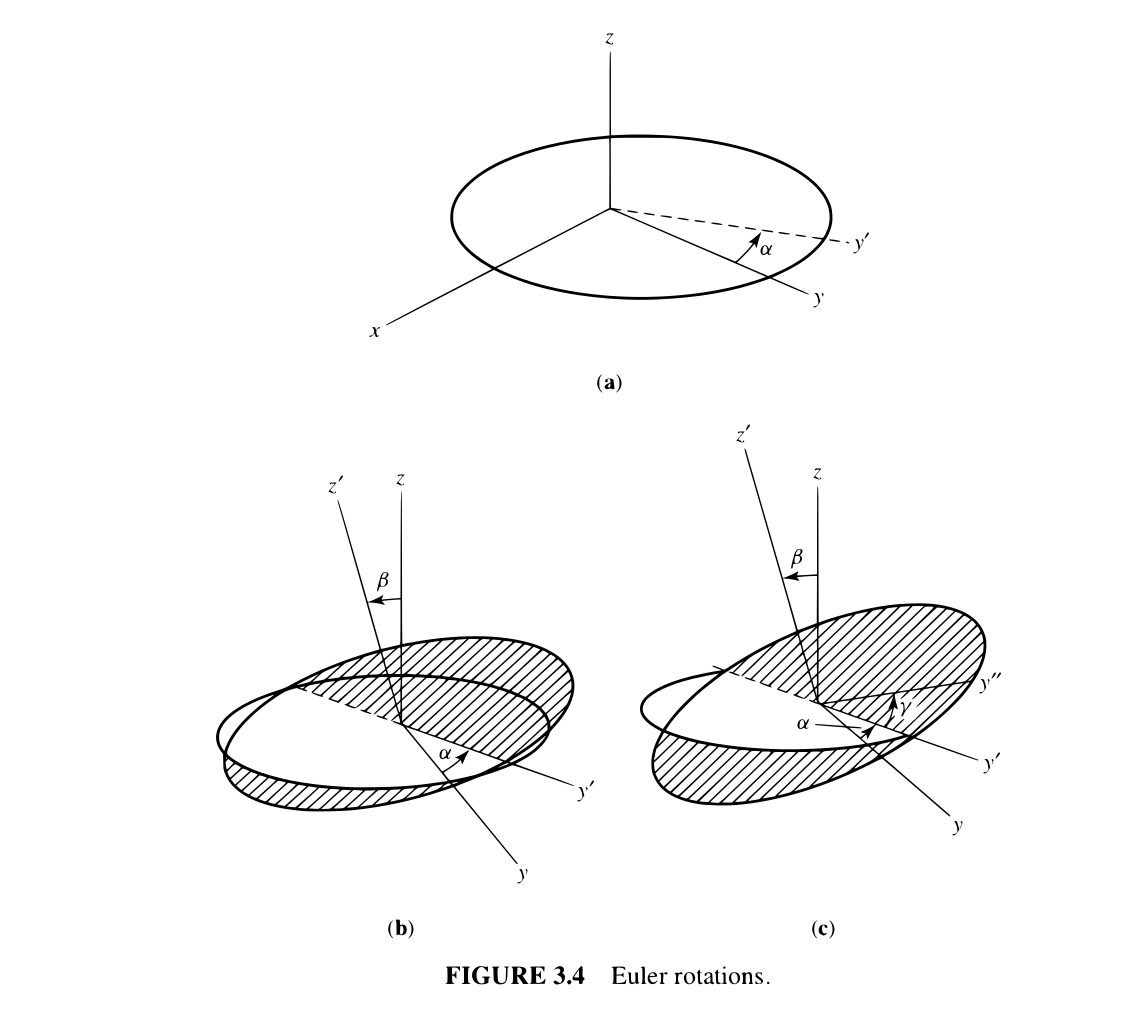
\includegraphics[width=0.65\textwidth]{figures/Euler Rotation.png}
    \caption{Euler Rotations}
\end{figure}
Having obtained the matrix elements of $J_z$ and $J_\pm$, we are now in a position to
study the matrix elements of the rotation operator $\mathscr{D}(R)$. If a rotation $R$ is specified
by $\hat{\mathbf{n}}$ and $\phi$, we can define its matrix elements by
\begin{equation}
    \mathscr{D}^{(j)}_{m'm}(R)=\bra{j,m'}\exp\left(\frac{-\ii \mathbf{J}\cdot\hat{\mathbf{n}}\phi}{\hbar}\right)\ket{j,m}.
\end{equation}
These matrix elements are sometimes called \textbf{Wigner functions}.
In Euler Rotations, the rotation operator is defined by
\begin{equation}
    \begin{aligned}
        &\mathscr{D}^{(j)}_{m'm}(\alpha,\beta,\gamma)\\
        =&\bra{j,m'}\exp\left(\frac{-\ii J_z \alpha}{\hbar }\right)\exp\left(\frac{\ii J_y \beta}{\hbar}\right)\exp\left(\frac{-\ii J_z \gamma}{\hbar}\right)\ket{j,m}\\
        =&\ee ^{-\ii\left( m' \alpha+m\gamma\right)}\bra{j,m'}\exp\left(\frac{-\ii J_y \beta}{\hbar}\right)\ket{j,m}.
    \end{aligned}
\end{equation}
We denote nontrivial part as 
\begin{equation}
    d^{(j)}_{m'm}(\beta)=\bra{j,m'}\exp\left(\frac{-\ii J_y \beta}{\hbar}\right)\ket{j,m}.
\end{equation}
Since 
\begin{equation}
    \left[\mathbf{J}^2,\mathscr{D}(R)\right]=0,
\end{equation}
any state $\ket{j,m}$ after a rotation $R$ is also an eigenket of $\mathbf{J}^2$, and its eigenvalue is still $j(j+1)\hbar^2$.

To find the amplitude for being found in $\ket{j,m}$ , we simply expand the rotated state as follows:
\begin{equation}
    \mathscr{D}(R)\ket{j,m}=\sum_{m'}\ket{j,m'}\bra{j,m'}\mathscr{D}(R)\ket{j,m}=\sum_{m'}\ket{j,m'}\mathscr{D}^{(j)}_{m'm}(R).
\end{equation}


\subsection{Spherical Harmonics}
\footnote{\href{run:Spherical Functions.pdf alias}{Spherical Functions.}}
Let us consider a problem with spherical symmetry, we can consider
\begin{equation}
    \bra{\hat{\mathbf{n}}}\ket{l,m}=Y_l^m(\hat{\mathbf{n}})=Y_l^m\left(\theta,\phi\right),
\end{equation}
where we have defined a \textbf{direction eigenket} $\ket{\hat{\mathbf{n}}}$.

By \eqref{13.34}, we have 
\begin{equation}\label{13.44}
    -\ii \hbar \frac{\pa}{\pa \phi}Y_l^m\left(\theta,\phi\right)=m\hbar Y_l^m\left(\theta,\phi\right),
\end{equation}
\begin{equation}
    \left[\frac{1}{\sin \theta}\frac{\pa}{\pa \theta}\left(\sin\theta\frac{\pa}{\pa \theta}\right)+\frac{1}{\sin^2\theta}\frac{\pa^2}{\pa \phi^2}+l\left(l+1\right)\right]Y_l^m=0.
\end{equation}
By 
\begin{equation}
    \bra{l',m'}\ket{l,m}=\delta_{ll'}\delta_{mm'},
\end{equation}
we obtain,
\begin{equation}\label{13.48}
    \int_{0}^{2\pi}\dd{\phi}\int_{-1}^{1}\dd{(\cos\theta)}{Y_{l'}^{m'}}^*\left(\theta,\phi\right)Y^m_l\left(\theta,\phi\right)=\delta_{ll'}\delta_{mm'}.
\end{equation}
\eqref{13.44} implies that the $\phi$-independence $Y_l^m\left(\theta,\phi\right)$ must behave like $\ee^{\ii m \phi}$. By \eqref{13.20},
\begin{equation}
    \left[\ii \frac{\pa }{\pa \theta}-\cot\theta\frac{\pa}{\pa \phi}\right]\braket{\hat{\mathbf{n}}}{l,l}=0.
\end{equation}
So, 
\begin{equation}
    Y_l^l\left(\theta,\phi\right)=c_l\ee^{\ii l\phi}\sin^l\theta.
\end{equation}
Use \eqref{13.48} to normalize,
\begin{equation}
    \int_{0}^{\pi}\sin^{2l}\theta \sin\theta \dd{\theta}=B\left(l+1,\frac{1}{2}\right)=\frac{\Gamma\left(l+1\right)\Gamma\left(\frac{1}{2}\right)}{\Gamma\left(l+\frac{3}{2}\right)}.
\end{equation}
Then we can use the ladder operator to get $Y_l^m$. Check details in the reference.
\end{document}